\documentclass[11pt]{article}

% ---- packages ----
\usepackage[margin=1in]{geometry}
\usepackage{amsmath,amssymb,amsthm}
\usepackage{mathtools}
\usepackage{algorithm}
\usepackage{algpseudocode}
\usepackage{hyperref}
\usepackage{cleveref}
\usepackage{graphicx}
\usepackage{booktabs}
\usepackage{enumitem}
\usepackage{xcolor}
\usepackage{tikz}
\usetikzlibrary{positioning, arrows.meta, calc}
\usepackage[numbers]{natbib}

% ---- theorem environments ----
\newtheorem{definition}{Definition}[section]
\newtheorem{assumption}{Assumption}[section]
\newtheorem{lemma}{Lemma}[section]
\newtheorem{theorem}{Theorem}[section]
\newtheorem{proposition}{Proposition}[section]
\newtheorem{corollary}{Corollary}[section]
\newtheorem{remark}{Remark}[section]
\newtheorem{example}{Example}[section]
\newtheorem{experiment}{Experiment}[section]

% ---- macros ----
\newcommand{\negl}{\mathsf{negl}}
\newcommand{\poly}{\mathsf{poly}}
\newcommand{\calA}{\mathcal{A}}
\newcommand{\calC}{\mathcal{C}}
\newcommand{\calM}{\mathcal{M}}
\newcommand{\calX}{\mathcal{X}}
\newcommand{\calR}{\mathcal{R}}
\newcommand{\calY}{\mathcal{Y}}
\newcommand{\Prove}{\mathsf{Prove}}
\newcommand{\Verify}{\mathsf{Verify}}
\newcommand{\Cost}{\mathsf{Cost}}

\newcommand{\TODO}[1]{\textcolor{red}{\textbf{[TODO: #1]}}}
\newcommand{\thomas}[1]{\textcolor{red}{\textbf{Thomas:} #1}}

% ---- title ----
\title{On the Computational Independence of ML Inference\\for PoML Consensus}
\author{Thomas Wong}

\begin{document}
\maketitle

% \begin{abstract}
% The security of the Proof-of-ML-Inference (PoML) consensus mechanism relies on a reduction to the Bitcoin backbone protocol, which models hash computation as queries to a $q$-bounded random oracle. A key implicit assumption in this model is that each oracle query incurs \emph{uniform computational cost}: the effort required is independent of the query input, and knowledge of one query's output confers no advantage in computing another. In PoML, each ``query'' corresponds to the generation of an ML inference--proof pair. We must therefore establish that inference--proof generation exhibits analogous uniformity properties. This note formalises the necessary assumptions, introduces the \emph{Computational Independence Assumption} (CIA) for neural network inference, proposes an experimental methodology to validate it using BigGAN as a representative model, and shows how the CIA, together with properties of the ZKP proving system, suffices to justify the $q_{\mathrm{ML}}$-bounded random oracle abstraction used in the PoML security analysis.
% \end{abstract}

% ============================================================
\section{Background}
\label{sec:background}
% ============================================================

The security of Bitcoin's consensus mechanism is established through the \emph{backbone protocol} analysis of Garay, Kiayias, and Leonardos~\cite{garay2015bitcoin}. The analysis operates in a synchronous model where time proceeds in discrete rounds, and miners interact with a hash function $H(\cdot)$ modelled as a \emph{random oracle}. The central abstraction is the \emph{$q$-bounded random oracle model}: in each round, every flat-model party is permitted at most $q$ queries to $H(\cdot)$. Each query evaluates $H(\mathit{ctr}, \cdot)$ for some counter value $\mathit{ctr}$ and checks whether the output falls below a difficulty target~$T$.

This abstraction implicitly relies on two properties of hash function evaluation that are inherited from the random oracle idealisation:

\begin{enumerate}[label=(\roman*)]
    \item \textbf{Uniform query cost.} Every evaluation of $H(\cdot)$ requires the same computational effort, regardless of the input. There is no class of inputs for which $H$ can be evaluated faster, nor any input for which evaluation is disproportionately expensive. This property ensures that the bound~$q$ faithfully captures a party's computational budget per round.

    \item \textbf{Query independence.} Knowledge of $H(x)$---including any intermediate state arising during its computation---provides no computational advantage when evaluating $H(x')$ for $x' \neq x$. Each query is, in effect, an independent Bernoulli trial. This property ensures that the random variables $X_i, Y_i, Z_i$ in the backbone analysis (counting successful, uniquely successful, and adversarially successful rounds) are independent across queries.
\end{enumerate}

For SHA-256 as used in Bitcoin, both properties hold by the standard assumption that SHA-256 is well-modelled by a random oracle. Each hash evaluation traverses a fixed sequence of bitwise operations and modular additions whose count depends only on the message length (which is fixed in PoW), not on the message content. The internal compression function processes each block identically, and no known structural shortcut allows relating the outputs of two distinct inputs.

\paragraph{The PoML setting.}
In PoML, the role of hash evaluation is replaced by the generation of an \emph{inference--proof pair}: given a machine learning model $M_\theta$ and inputs $(x, r)$, a miner computes $y = M_\theta(x, r)$ and generates a zero-knowledge proof $\pi$ attesting to correct execution. The miner then evaluates a lottery $H_i = H(B_{\mathrm{header}} \| \pi_1 \| \cdots \| \pi_i)$ and checks whether $H_i < D$ for a global difficulty parameter~$D$. Each completed inference--proof pair yields exactly one lottery ticket.

We denote by $q_{\mathrm{ML}}$ the number of inference--proof pairs that a single flat-model party can complete per round. For the PoML security reduction to the backbone protocol, we require that $q_{\mathrm{ML}}$ faithfully models each party's computational budget---analogous to the role of $q$ in the backbone. This requires establishing that inference--proof generation satisfies properties analogous to (i) and (ii) above. That is:

\begin{enumerate}[label=(\roman*$'$)]
    \item \textbf{Uniform inference--proof cost.} The computational cost of producing $(y, \pi)$ for input $(x, r)$ is (essentially) the same for all valid inputs $(x, r)$.
    \item \textbf{Inference--proof independence.} Having computed $(y, \pi)$ for input $(x, r)$, an adversary gains no significant computational advantage in producing $(y', \pi')$ for a different input $(x', r')$.
\end{enumerate}

The remainder of this note is devoted to formalising and justifying these two properties for the model class used in PoML.


% ============================================================
\section{The Model Class: Stochastic Denoising Models}
\label{sec:model-class}
% ============================================================

We restrict attention to the class of \emph{stochastic denoising diffusion models}---generative models whose sampling procedure iteratively refines random noise through a sequence of learned denoising steps interleaved with fresh stochastic perturbations.

\begin{definition}[Stochastic denoising model]
\label{def:model}
A \emph{stochastic denoising model} is a tuple
\[
    M_\theta \;=\; \bigl(f_\theta,\; T,\; (\sigma_t)_{t=2}^{T},\; d\bigr),
\]
where $f_\theta : \mathbb{R}^d \times \mathbb{R}^{d_c} \times [T] \to \mathbb{R}^d$ is a neural denoising network with parameters~$\theta$, $T \in \mathbb{N}$ is the number of denoising steps, $(\sigma_t)_{t=2}^{T}$ with $\sigma_t > 0$ is a fixed noise schedule, and $d$ is the latent dimension. We write $\calC$ for the class of all such models.
\end{definition}

\paragraph{Inputs.}
A model $M_\theta \in \calC$ takes as input a pair $(c, r)$, where:
\begin{itemize}[nosep]
    \item $c = e(x) \in \mathbb{R}^{d_c}$ is a \emph{precomputed conditioning embedding}, obtained by applying a public, deterministic embedding function $e : \calX \to \mathbb{R}^{d_c}$ to the conditioning input~$x$ (e.g., a text prompt or class label). The PoML protocol requires that miners compute $c = e(x)$ before inference--proof generation begins; the embedding cost is therefore external to the proved computation.
    \item $r \in \{0,1\}^\lambda$ is a \emph{random seed} that deterministically generates all stochasticity required during sampling. A pseudorandom generator $G : \{0,1\}^\lambda \to \mathbb{R}^{d \times T}$ (modelled as a random oracle in the security analysis) expands $r$ into the initial noise tensor $x_T \in \mathbb{R}^d$ and the per-step noise vectors $z_T, z_{T-1}, \ldots, z_2 \in \mathbb{R}^d$ used during the reverse process.
\end{itemize}

\paragraph{Denoising procedure.}
Given inputs $(c, r)$, the model executes $T$ denoising steps. At each step $t = T, T{-}1, \ldots, 2$:
\begin{equation}
\label{eq:denoise-step}
    x_{t-1} \;=\; f_\theta(x_t,\, c,\, t) \;+\; \sigma_t\, z_t,
\end{equation}
where $\sigma_t > 0$ is a fixed noise-schedule parameter and $z_t \in \mathbb{R}^d$ is the noise vector derived from the seed~$r$. At the final step ($t = 1$), the output is computed without noise: $y = f_\theta(x_1, c, 1)$. The model output is $y = M_\theta(c, r)$.

\paragraph{Building blocks of $f_\theta$.}
The denoising network $f_\theta$ is assembled from standard operations, each with arithmetic cost determined solely by architecture constants:
\begin{itemize}[nosep]
    \item \textbf{Convolutional layers:} Learned kernels with fixed spatial dimensions, channel counts, and stride.
    \item \textbf{Normalisation layers:} Group normalisation or layer normalisation, with conditioning parameters derived from $(c, t)$.
    \item \textbf{Element-wise activations:} SiLU/Swish, GeLU, or ReLU applied independently per element.
    \item \textbf{Attention layers:} Self-attention within spatial feature maps, and cross-attention between feature maps and the conditioning embedding~$c$.
    \item \textbf{Residual and skip connections:} Element-wise addition or concatenation of feature maps at matching resolutions.
\end{itemize}

\begin{figure}[t]
\centering
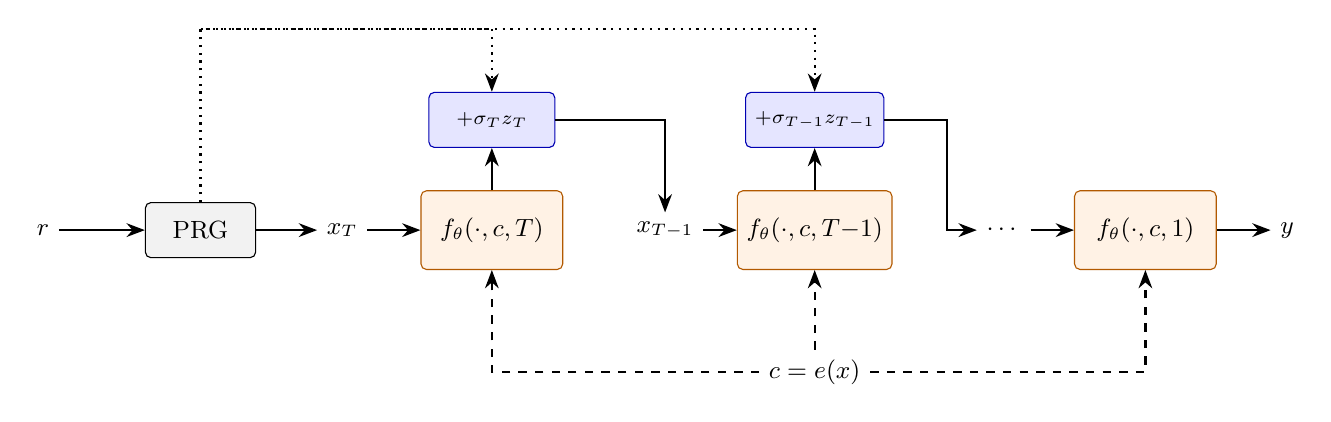
\begin{tikzpicture}[
    >=Stealth,
    font=\small,
    ubox/.style={draw=orange!70!black, rounded corners=2pt, minimum height=10mm,
                 minimum width=18mm, align=center, fill=orange!10, font=\small},
    nbox/.style={draw=blue!70!black, rounded corners=2pt, minimum height=7mm,
                 minimum width=16mm, align=center, fill=blue!10, font=\scriptsize},
]
  % Inputs
  \node (r) at (-1.8,0) {$r$};
  \node[draw, rounded corners=2pt, minimum height=7mm, minimum width=14mm,
       fill=gray!10, font=\small] (prg) at (0.2,0) {PRG};
  % x_T
  \node (xT) at (2.0,0) {$x_T$};
  % Step T: UNet + noise
  \node[ubox] (u1) at (3.9,0) {$f_\theta(\cdot, c, T)$};
  \node[nbox] (n1) at (3.9,1.4) {$+\sigma_T z_T$};
  % x_{T-1}
  \node (xTm1) at (6.1,0) {$x_{T{-}1}$};
  % Step T-1: UNet + noise
  \node[ubox] (u1b) at (8.0,0) {$f_\theta(\cdot, c, T{-}1)$};
  \node[nbox] (n1b) at (8.0,1.4) {$+\sigma_{T{-}1} z_{T{-}1}$};
  % dots and final
  \node (dots) at (10.4,0) {$\cdots$};
  \node[ubox] (u2) at (12.2,0) {$f_\theta(\cdot, c, 1)$};
  \node (y) at (14.0,0) {$y$};
  % Conditioning
  \node (c) at (8.0,-1.8) {$c = e(x)$};
  % Main path arrows
  \draw[thick,->] (r) -- (prg);
  \draw[thick,->] (prg) -- (xT);
  \draw[thick,->] (xT) -- (u1);
  \draw[thick,->] (u1) -- (n1);
  \draw[thick,->] (n1.east) -| (xTm1.north);
  \draw[thick,->] (xTm1) -- (u1b);
  \draw[thick,->] (u1b) -- (n1b);
  \draw[thick,->] (n1b.east) -| ++(0.8,-1.4) -- (dots);
  \draw[thick,->] (dots) -- (u2);
  \draw[thick,->] (u2) -- (y);
  % Conditioning arrows
  \draw[thick,->,dashed] (c) -| (u1.south);
  \draw[thick,->,dashed] (c) -- (u1b.south);
  \draw[thick,->,dashed] (c) -| (u2.south);
  % PRG outputs for noise
  \draw[thick,->,dotted] (prg.north) -- ++(0,2.2) -| (n1.north);
  \draw[thick,->,dotted] (prg.north) ++(0,2.2) -| (n1b.north);
\end{tikzpicture}

\smallskip
{\small\itshape The seed $r$ is expanded by a PRG into $x_T$ and per-step noise vectors $z_T, z_{T-1}, \ldots$\ (dotted). Each denoising step applies $f_\theta$ with conditioning $c = e(x)$ (dashed), then adds stochastic noise to produce the next state. The final step outputs~$y$ without noise.}

\caption{Sampling pipeline for a stochastic denoising model in~$\calC$.}
\label{fig:architecture}
\end{figure}

\paragraph{Key architectural properties.}
The class $\calC$ is defined by two structural requirements:
\begin{enumerate}[label=(\alph*)]
    \item \textbf{Static computational graph.} Each evaluation of $f_\theta(\cdot, c, t)$ traverses a fixed sequence of operations---convolutions, normalisations, element-wise activations, residual connections, and (optionally) self- and cross-attention layers---in a predetermined order with fixed tensor dimensions. No conditional branches, early exits, or input-dependent routing decisions occur within~$f_\theta$, and the noise injection in~\eqref{eq:denoise-step} is likewise a fixed-cost operation. This ensures uniform query cost (\Cref{subsec:uniform-cost}).
    \item \textbf{Per-step stochastic noise injection.} The defining feature that distinguishes stochastic DDPM-style sampling~\cite{ho2020ddpm} from deterministic variants (e.g., DDIM) is that at each step $t \geq 2$, independent Gaussian noise scaled by $\sigma_t > 0$ is added to the denoiser output. This is the structural property that drives the computational independence theorem (\Cref{sec:independence-thm}).
\end{enumerate}

\paragraph{Example: Stable Diffusion.}
Stable Diffusion v1-4~\cite{rombach2022ldm} is an instance of~$\calC$. The conditioning input $x$ is a text prompt, and $c = e(x)$ is computed by a frozen CLIP text encoder (external to the proved computation). The denoising network $f_\theta$ is a U-Net (${\sim}860$M parameters) operating in a compressed latent space ($d = 4 \times 64 \times 64 = 16{,}384$) over $T = 50$ steps using the DDPM noise schedule with $\sigma_t > 0$ for all $t \geq 2$.


% ============================================================
\section{Formalising the Required Properties}
\label{sec:properties}
% ============================================================

We formalise the two properties that inference--proof generation must satisfy for the $q_{\mathrm{ML}}$-bounded random oracle abstraction to hold.

% ---- Property 1 ----
\subsection{Uniform Query Cost}
\label{subsec:uniform-cost}

\begin{definition}[Arithmetic Cost]
\label{def:arith-cost}
Let $M_\theta = (f_\theta, T, (\sigma_t), d) \in \calC$. The \emph{architecture cost} of~$M_\theta$ is
\[
    \Cost(M_\theta) \;=\; T \cdot \Cost(f_\theta) \;+\; (T-1) \cdot \Cost(\text{noise}),
\]
where $\Cost(f_\theta)$ is the FLOP count of a single evaluation of the denoising network and $\Cost(\text{noise}) = \Theta(d)$ is the cost of the noise scaling and addition at each step. Since $f_\theta$ has a static computational graph (\Cref{sec:model-class}), both terms are architecture constants independent of the input values.
\end{definition}

\begin{lemma}[Uniform query cost]
\label{lem:uniform-cost}
Let $\Cost(M_\theta, c, r)$ be the arithmetic cost (FLOP count) of evaluating $M_\theta$ on input $(c, r)$. Every model $M_\theta \in \calC$ satisfies $\Cost(M_\theta, c, r) = \Cost(M_\theta)$ for all $(c, r)$.
\end{lemma}

\begin{proof}
By definition of~$\calC$, every denoising step executes the same static computational graph with fixed operation counts. The number of steps $T$ and the noise schedule $(\sigma_t)$ are architecture constants, and no component depends on the numerical values of $(c, r)$.
\end{proof}

% ---- Property 2 ----
\subsection{Computational Independence}
\label{subsec:independence}

The second property is more subtle and constitutes the main focus of this note. We formalise it through the following experiment, which captures an adversary's ability to exploit prior computations.

\begin{experiment}[Inference--Proof Amortisation Game]
\label{exp:amortisation}
Let $\lambda$ be a security parameter, let $M_\theta \in \calC$, and let $(\Prove, \Verify)$ be a zero-knowledge proof system for correct inference under~$M_\theta$. The game $\mathsf{Amort}_{\calA, M_\theta}(\lambda)$ proceeds as follows:

\begin{enumerate}[nosep]
    \item The challenger samples $r_1, r_2 \overset{\mathrm{i.i.d.}}{\sim} \{0,1\}^\lambda$.
    \item \textbf{Round 1.} The challenger sends $r_1$ and a conditioning embedding $c \in \mathbb{R}^{d_c}$ to $\calA$. The adversary outputs $(y_1, \mathsf{stmt}_1, \pi_1)$, and the challenger verifies that $y_1 = M_\theta(c, r_1)$ and $\Verify(\mathsf{CRS}, \mathsf{stmt}_1, \pi_1) = 1$.
    \item \textbf{Round 2.} The challenger sends $r_2$ to $\calA$. The adversary may adaptively choose a new embedding $c'$ and outputs $(y_2, \mathsf{stmt}_2, \pi_2)$. The challenger verifies analogously.
    \item Let $T_2$ be the adversary's computational cost in round~2, and $T^*$ the expected honest cost.
\end{enumerate}

\noindent The \emph{amortisation advantage} is $\mathsf{Adv}^{\mathrm{amort}}_{\calA, M_\theta}(\lambda) = 1 - T_2 / T^*$.
\end{experiment}

\begin{definition}[Amortisation Resistance]
\label{def:amort-resist}
Inference--proof generation for $M_\theta$ is \emph{$\epsilon$-amortisation resistant} if for all PPT adversaries $\calA$:
\[
    \Pr\!\left[\mathsf{Adv}^{\mathrm{amort}}_{\calA, M_\theta}(\lambda) > \epsilon \right] \leq \negl(\lambda).
\]
\end{definition}


% ============================================================
\section{Computational Independence of Stochastic Denoising}
\label{sec:independence-thm}
% ============================================================

We now argue that stochastic denoising models satisfy computational independence due to the noise injection of models.

\subsection{Quantization in ZKP Circuits}
\label{subsec:quantization}

Zero-knowledge proof systems for neural network inference (e.g., ezkl~\cite{ezkl2024}, ZKML~\cite{chen2024zkml}) operate over finite fields and represent all intermediate values via fixed-point quantization: a global scale factor $s = 2^k$ maps each floating-point value $v \in \mathbb{R}$ to the integer $\hat{v} = \lfloor v \cdot s \rceil \in \mathbb{Z}$.

\begin{definition}[Quantization Resolution]
\label{def:quant-res}
The \emph{quantization resolution} is $\delta = 2^{-k}$. Two values $v_1, v_2 \in \mathbb{R}$ are \emph{quantization-equivalent} if $|v_1 - v_2| < \delta/2$.
\end{definition}

Typical ZKML implementations use $k \in [10, 18]$, yielding $\delta \in [2^{-18}, 2^{-10}]$.

\subsection{$\delta$-Reusable State}
\label{subsec:reusable}

\begin{definition}[$\delta$-Reusable State]
\label{def:reusable}
The denoising state $x_t \in \mathbb{R}^d$ is \emph{$\delta$-reusable} between two executions with seeds $r, r'$ if
\[
    \bigl\lfloor x_{t,j}(r) \cdot s \bigr\rceil = \bigl\lfloor x_{t,j}(r') \cdot s \bigr\rceil \quad \text{for all } j = 1, \ldots, d.
\]
If $x_t$ is $\delta$-reusable, the ZKP circuit for step~$t$ receives identical quantized inputs and the computation of $f_\theta(x_t, c, t)$ can potentially be skipped.
\end{definition}


\subsection{Negligible Reusability Theorem}
\label{subsec:main-theorem}

The core insight is that per-step noise injection makes computation reuse negligibly probable, regardless of the model weights~$\theta$. The argument uses only the anti-concentration property of Gaussian distributions.

\begin{lemma}[Gaussian anti-concentration]
\label{lem:anti-conc}
Let $W \sim \mathcal{N}(0, \sigma^2)$ with $\sigma > 0$. For any $a \in \mathbb{R}$ and any $\delta > 0$:
\[
    \Pr\!\bigl[|a + W| \leq \delta/2\bigr] \;\leq\; \frac{\delta}{\sigma\sqrt{2\pi}}.
\]
\end{lemma}

\begin{proof}
The density of $a + W$ is bounded above by $\frac{1}{\sigma\sqrt{2\pi}}$, so $\Pr[|a + W| \leq \delta/2] \leq \delta \cdot \frac{1}{\sigma\sqrt{2\pi}}$.
\end{proof}

\begin{theorem}[Negligible reusability for stochastic denoising]
\label{thm:cia}
Let $M_\theta \in \calC$ with $T$ denoising steps, latent dimension~$d$, and noise schedule $\sigma_t > 0$ for $t = T, \ldots, 2$. Let $\sigma_{\min} = \min_{t \geq 2} \sigma_t$ and suppose $\delta < 2\sigma_{\min}\sqrt{2\pi}$. For two independent seeds $r, r' \overset{\mathrm{i.i.d.}}{\sim} \{0,1\}^\lambda$:
\[
    \Pr\!\bigl[\,\exists\, t \in \{1, \ldots, T\} :\; x_t(r) \text{ is } \delta\text{-reusable with } x_t(r')\bigr] \;\leq\; T \cdot \left(\frac{\delta}{2\sigma_{\min}\sqrt{\pi}}\right)^{\!d}.
\]
In particular, for any fixed $\delta$ and $\sigma_{\min} > 0$, this probability is negligible in the latent dimension~$d$.
\end{theorem}

\begin{proof}
We bound the probability that any single step's input state is $\delta$-reusable, then apply a union bound over $T$ steps.

\paragraph{Step $T$ (initial noise).}
The states $x_T(r)$ and $x_T(r')$ are independent samples from $\mathcal{N}(0, I_d)$. For each component~$j$, the difference $x_{T,j}(r) - x_{T,j}(r') \sim \mathcal{N}(0, 2)$. By \Cref{lem:anti-conc} with $a = 0$ and $\sigma = \sqrt{2}$:
\[
    \Pr\!\bigl[|x_{T,j}(r) - x_{T,j}(r')| \leq \delta/2\bigr] \;\leq\; \frac{\delta}{2\sqrt{\pi}}.
\]
Since the components are independent, the probability that \emph{all} $d$ components are quantization-equivalent is at most $\bigl(\delta/(2\sqrt{\pi})\bigr)^d$.

\paragraph{Steps $t = T{-}1, \ldots, 1$.}
From~\eqref{eq:denoise-step}, $x_t = f_\theta(x_{t+1}, c, t{+}1) + \sigma_{t+1}\, z_{t+1}$ (for $t \leq T{-}1$), where $z_{t+1}(r)$ and $z_{t+1}(r')$ are independent $\mathcal{N}(0, I_d)$ vectors derived from their respective seeds. For each component~$j$:
\[
    x_{t,j}(r) - x_{t,j}(r') \;=\; \underbrace{f_\theta(x_{t+1}(r), c, t{+}1)_j - f_\theta(x_{t+1}(r'), c', t{+}1)_j}_{=:\, a_j} \;+\; \sigma_{t+1}\bigl[z_{t+1,j}(r) - z_{t+1,j}(r')\bigr].
\]
Conditioned on $(x_{t+1}(r), x_{t+1}(r'))$, the term $a_j$ is a deterministic constant and $z_{t+1,j}(r) - z_{t+1,j}(r') \sim \mathcal{N}(0, 2)$. By \Cref{lem:anti-conc} with $a = a_j$ and $\sigma = \sigma_{t+1}\sqrt{2}$:
\[
    \Pr\!\bigl[|x_{t,j}(r) - x_{t,j}(r')| \leq \delta/2 \;\big|\; x_{t+1}(r), x_{t+1}(r')\bigr] \;\leq\; \frac{\delta}{2\sigma_{t+1}\sqrt{\pi}}\,.
\]
Since the noise components $z_{t+1,j}$ are independent across~$j$ (conditioned on $x_{t+1}$), the probability that all $d$ components are simultaneously quantization-equivalent is at most $\bigl(\delta/(2\sigma_{t+1}\sqrt{\pi})\bigr)^d$. This bound holds for every value of $(x_{t+1}(r), x_{t+1}(r'))$ and hence unconditionally.

\paragraph{Union bound.}
Taking a union bound over all $T$ steps, and using $\sigma_{t+1} \geq \sigma_{\min}$ for $t \leq T{-}1$ and the initial noise effective standard deviation $1 \geq \sigma_{\min}$:
\[
    \Pr[\exists\, t : x_t \text{ is } \delta\text{-reusable}] \;\leq\; T \cdot \left(\frac{\delta}{2\sigma_{\min}\sqrt{\pi}}\right)^{\!d}. \qedhere
\]
\end{proof}


\begin{example}[Numerical instantiation]
\label{rem:numerical}
For Stable Diffusion v1-4 with $d = 16{,}384$, $T = 50$, $\sigma_{\min} \approx 0.01$ (linear noise schedule), and $\delta = 2^{-10} \approx 10^{-3}$: the per-component probability is $\delta/(2\sigma_{\min}\sqrt{\pi}) \approx 0.028$, and the per-step bound is $0.028^{16{,}384} < 10^{-25{,}000}$. Even after the union bound over $T = 50$ steps, the probability remains astronomically small. The condition $\delta < 2\sigma_{\min}\sqrt{2\pi} \approx 0.05$ is satisfied for all standard quantization precisions $k \geq 5$.
\end{example}

\begin{remark}[No partial reuse within $f_\theta$]
\label{rem:no-partial-reuse}
One might ask whether an adversary could reuse \emph{sub-computations} within $f_\theta$---for instance, reusing early-layer activations when two inputs $x_t$ and $x_t'$ are close but not identical. While we cannot formally claim this to be impossible, the chances of reusing sub-computations are close to negligible, especially considering the ZKP setting. The proof attests to the correctness of \emph{every intermediate wire value} in the arithmetic circuit implementing $f_\theta$. Each wire value is a deterministic function of the circuit input~$x_t$, so distinct inputs produce distinct execution traces. In order to reuse computation, the intermediate activations must be $\delta$-reusable, which is shown in section~\ref{sec:experiments} as highly unlikely. We therefore make the assumption that computation of $f_\theta$ is not reusable for distinct inputs.
\end{remark}

\begin{figure}[t]
\centering
\includegraphics[width=0.7\textwidth]{plots/compare.png}
\caption{Visual illustration of activation divergence. Two images generated by Stable Diffusion v1.4 with the same prompt \textit{``an astronaut riding a horse in a photorealistic style''} but seeds differing by a small perturbation ($\eta \sim \mathcal{N}(0, 0.01 \cdot I)$ added to the initial latent). The outputs differ substantially in composition, colour, and fine detail, reflecting the rapid divergence of intermediate activations predicted by \Cref{thm:cia}.}
\label{fig:activation-divergence}
\end{figure}
% ============================================================
\section{Empirical Validation}
\label{sec:experiments}
% ============================================================

\Cref{thm:cia} establishes negligible reusability as a theoretical guarantee. We complement this with empirical measurements of activation divergence in Stable Diffusion v1-4~\cite{rombach2022ldm} to confirm that the divergence predicted by the theorem is observable in practice, even under the smallest perturbations.

\paragraph{Setup.}
Fix a text prompt~$x$ and a base seed~$r$ producing initial noise $x_T \sim \mathcal{N}(0, I_d)$.  Construct perturbed seeds by adding $\eta \sim \mathcal{N}(0, \sigma^2 I_d)$ to the initial noise, for perturbation scales $\sigma \in \{0.001, 0.01, 0.1, 0.5, 1.0\}$.  We also include a baseline where the seed~$r'$ is sampled independently.  For each perturbation scale we draw $N = 1{,}000$ base inputs and record all intermediate activations at every denoising step.

\paragraph{Metrics.}
At each denoising step~$t$ we compute the cosine similarity $s_t = h_t(r) \cdot h_t(r') / (\|h_t(r)\|_2 \|h_t(r')\|_2)$ between base and perturbed activations, and the minimum $L^\infty$ distance $\|h_t(r) - h_t(r')\|_\infty$ across all steps and samples.  A step is non-$\delta$-reusable whenever $\|h_t(r) - h_t(r')\|_\infty \geq \delta/2$.

\begin{figure}[t]
\centering
\includegraphics[width=0.55\textwidth]{results/sd_cosine_sim_vs_step.pdf}
\caption{Cosine similarity between base and perturbed activations for Stable Diffusion, plotted against denoising step.  Each curve corresponds to a perturbation scale~$\sigma$; shaded bands show $\pm 1$ standard deviation over $N = 1{,}000$ samples.  The dashed line is the independent-seed baseline.  Cosine similarity decreases with depth, confirming rapid activation divergence consistent with \Cref{thm:cia}.}
\label{fig:cosine_sim}
\end{figure}

\paragraph{Results.}
\Cref{fig:cosine_sim} shows that cosine similarity decreases steadily with denoising depth for all perturbation scales, converging toward the independent baseline.  This confirms that even with identical conditioning~$c = e(x)$, intermediate activations diverge rapidly---consistent with the per-step noise injection mechanism underlying \Cref{thm:cia}.

\Cref{tab:min-linf} reports the minimum $L^\infty$ distance across all samples and denoising steps.  Even at the smallest perturbation ($\sigma = 0.001$), the minimum distance is $D_\infty = 2.93 \times 10^{-3}$, exceeding $\delta/2 = 2^{-(k+1)}$ for all $k \leq 8$.  For $\sigma \geq 0.01$, all activations are non-$\delta$-reusable for the full ZKML precision range $k \in [10, 18]$.

\begin{table}[t]
  \centering
  \caption{Minimum $L^\infty$ distance between base and perturbed activations for Stable Diffusion across all $N = 1{,}000$ samples and denoising steps.}
  \label{tab:min-linf}
  \begin{tabular}{lr}
    \toprule
    $\boldsymbol{\sigma}$ & \textbf{Min $L^\infty$ distance} \\
    \midrule
    $0.001$ & $0.00293$ \\
    $0.010$ & $0.02832$ \\
    $0.100$ & $0.28076$ \\
    $0.500$ & $0.75488$ \\
    $1.000$ & $2.57617$ \\
    \bottomrule
  \end{tabular}
\end{table}

These empirical observations corroborate the theoretical bound: the stochastic noise injection at each denoising step produces activation differences that far exceed any reasonable quantization threshold, rendering computation reuse infeasible.
% ============================================================
\section{From Negligible Reusability to Amortisation Resistance}
\label{sec:full-argument}
% ============================================================

We now show that \Cref{thm:cia}, together with the structure of the PoML proof system, implies amortisation resistance (\Cref{def:amort-resist}) for the full inference--proof pair.

\begin{theorem}[Inference--proof amortisation resistance]
\label{thm:combined}
Let $M_\theta \in \calC$ satisfy the conditions of \Cref{thm:cia}, and let the proof system be a sound SNARK. Then the inference--proof generation for $M_\theta$ is $\negl(\lambda)$-amortisation resistant.
\end{theorem}

\begin{proof}
We bound the adversary's savings on each component of round~2.

\paragraph{Inference.}
In round~2 of the amortisation game (\Cref{exp:amortisation}), the adversary receives a fresh seed~$r_2$ independent of~$r_1$. By \Cref{thm:cia}, the probability that \emph{any} denoising step's input state is $\delta$-reusable between the two seeds is at most $T \cdot (\delta/(2\sigma_{\min}\sqrt{\pi}))^d = \negl(\lambda)$. Therefore, with overwhelming probability, the adversary must recompute all $T$ evaluations of $f_\theta$ from scratch, yielding $T_2^{\mathrm{inf}} \geq (1 - \negl(\lambda)) \cdot T^{*,\mathrm{inf}}$.

\paragraph{Proof generation.}
Since the quantized intermediate activations differ at every denoising step with overwhelming probability, the SNARK witnesses for rounds~1 and~2 differ in $\Omega(N)$ field elements (where $N$ is the total witness size). Moreover, PoML requires each proof statement to embed the hash of the previous proof, so the round-2 statement differs from round~1 with probability $1 - \negl(\lambda)$. A SNARK prover with a different witness and statement cannot reuse prior proof computation (the prover's internal polynomial commitments and evaluation proofs are witness-dependent), so $T_2^{\mathrm{pf}} \geq (1 - \negl(\lambda)) \cdot T^{*,\mathrm{pf}}$.

\paragraph{Combining.}
The total round-2 cost satisfies $T_2 \geq (1 - \negl(\lambda)) \cdot T^*$, yielding
\[
    \mathsf{Adv}^{\mathrm{amort}}_{\calA, M_\theta}(\lambda) \;\leq\; \negl(\lambda). \qedhere
\]
\end{proof}

\paragraph{Discussion.}
Since the conditioning embedding $c = e(x)$ is precomputed externally by the miner and excluded from the proved computation, the model~$M_\theta$ contains no deterministically reusable component. Combined with the per-step noise injection, the amortisation advantage is negligible. Each flat-model party can generate at most $q_\mathsf{ML}$ inference--proof pairs per round, with no opportunity to amortise computation across different seeds.

% ============================================================
% REFERENCES
% ============================================================
\bibliographystyle{plainnat}

\begin{thebibliography}{10}

\bibitem{garay2015bitcoin}
Juan~A. Garay, Aggelos Kiayias, and Nikos Leonardos.
\newblock The {B}itcoin backbone protocol: Analysis and applications.
\newblock In \emph{Advances in Cryptology -- EUROCRYPT 2015}, volume 9057 of LNCS, pages 281--310. Springer, 2015.
\newblock Full version: IACR ePrint 2014/765.

\bibitem{garay2017variable}
Juan~A. Garay, Aggelos Kiayias, and Nikos Leonardos.
\newblock The {B}itcoin backbone protocol with chains of variable difficulty.
\newblock In \emph{Advances in Cryptology -- CRYPTO 2017}, volume 10401 of LNCS, pages 291--312. Springer, 2017.

\bibitem{goodfellow2014gan}
Ian~J. Goodfellow, Jean Pouget-Abadie, Mehdi Mirza, Bing Xu, David Warde-Farley, Sherjil Ozair, Aaron Courville, and Yoshua Bengio.
\newblock Generative adversarial nets.
\newblock In \emph{Advances in Neural Information Processing Systems (NeurIPS)}, pages 2672--2680, 2014.

\bibitem{brock2019biggan}
Andrew Brock, Jeff Donahue, and Karen Simonyan.
\newblock Large scale {GAN} training for high fidelity natural image synthesis.
\newblock In \emph{International Conference on Learning Representations (ICLR)}, 2019.

\bibitem{karras2020stylegan2}
Tero Karras, Samuli Laine, Miika Aittala, Janne Hellsten, Jaakko Lehtinen, and Timo Aila.
\newblock Analyzing and improving the image quality of {StyleGAN}.
\newblock In \emph{CVPR}, pages 8110--8119, 2020.

\bibitem{sauer2023stylegan-t}
Axel Sauer, Tero Karras, Samuli Laine, Andreas Geiger, and Timo Aila.
\newblock {StyleGAN-T}: Unlocking the power of {GANs} for fast large-scale text-to-image synthesis.
\newblock In \emph{ICML}, 2023.

\bibitem{kang2023gigagan}
Minguk Kang, Jun-Yan Zhu, Richard Zhang, Jaesik Park, Eli Shechtman, Sylvain Paris, and Taesung Park.
\newblock Scaling up {GANs} for text-to-image synthesis.
\newblock In \emph{CVPR}, 2023.

\bibitem{ho2020ddpm}
Jonathan Ho, Ajay Jain, and Pieter Abbeel.
\newblock Denoising diffusion probabilistic models.
\newblock In \emph{Advances in Neural Information Processing Systems (NeurIPS)}, pages 6840--6851, 2020.

\bibitem{rombach2022ldm}
Robin Rombach, Andreas Blattmann, Dominik Lorenz, Patrick Esser, and Bj{\"o}rn Ommer.
\newblock High-resolution image synthesis with latent diffusion models.
\newblock In \emph{CVPR}, pages 10684--10695, 2022.

\bibitem{song2023consistency}
Yang Song, Prafulla Dhariwal, Mark Chen, and Ilya Sutskever.
\newblock Consistency models.
\newblock In \emph{International Conference on Machine Learning (ICML)}, pages 32211--32252. PMLR, 2023.

\bibitem{chen2024zkml}
Bing-Jyue Chen, Suppakit Waiwitlikhit, Ion Stoica, and Daniel Kang.
\newblock {ZKML}: An optimizing system for {ML} inference in zero-knowledge proofs.
\newblock In \emph{EuroSys '24}, pages 560--574. ACM, 2024.

\bibitem{ezkl2024}
Zkonduit Inc.
\newblock ezkl: Easy zero-knowledge inference.
\newblock \url{https://github.com/zkonduit/ezkl}, 2024.

\bibitem{groth16}
Jens Groth.
\newblock On the size of pairing-based non-interactive arguments.
\newblock In \emph{EUROCRYPT 2016}, volume 9666 of LNCS, pages 305--326. Springer, 2016.

\bibitem{ali2020puzzles}
Isra~Mohamed Ali, Maurantonio Caprolu, and Roberto Di~Pietro.
\newblock Foundations, properties, and security applications of puzzles: A survey.
\newblock \emph{ACM Computing Surveys}, 53(4):1--38, 2020.

\bibitem{fitzi2022ofelimos}
Matthias Fitzi, Aggelos Kiayias, Giorgos Panagiotakos, and Alexander Russell.
\newblock Ofelimos: Combinatorial optimization via proof-of-useful-work---a provably secure blockchain protocol.
\newblock In \emph{CRYPTO 2022}, volume 13509 of LNCS, pages 339--369. Springer, 2022.

\bibitem{fvcore}
Facebook Research.
\newblock fvcore: {FAIR} computer vision library.
\newblock \url{https://github.com/facebookresearch/fvcore}, 2021.

\end{thebibliography}

\end{document}